\documentclass[twocolumn]{article}

% Packages - all std in minimal LaTeX distributions
\usepackage{amsmath}
\usepackage{graphicx}



\title{Systematic Interaction Mining in Workforce Analytics:\\An Exhaustive Multi-Outcome, Multi-Model Empirical Evaluation}

\author{
    Naydhurve3$^\ast$ \\
    \small $^\ast$github.com/Naydhurve3/WorkForce-Data-Analysis
}

\date{}

\begin{document}

\twocolumn[
\begin{@twocolumnfalse}
\maketitle
\begin{abstract}
Workforce analytics has become a critical tool for organizations seeking to understand employee behavior, improve retention, and optimize human resource decisions. While much research has focused on predicting individual outcomes such as attrition, limited work has systematically examined how feature interactions influence multiple workforce outcomes simultaneously. This paper presents a comprehensive framework for exhaustive pairwise interaction mining in workforce data, evaluating 1,755 feature-pair combinations across five outcomes using three model families (Logistic Regression, Random Forest, XGBoost). We introduce a novel \textit{Interaction Impact Score} that combines mutual information, outcome differential, and segment size to quantify and rank interaction strength. All predictive results are reported as 5-fold cross-validation means $\pm$ standard deviations. Our results identify strong, statistically significant interactions---the strongest being JobFamily $\times$ DepartmentType predicting PayZone (impact score 181.3)---and reveal a heavy-tailed Pareto distribution where 3.1\% of pairs drive 80\% of total impact. However, adding interaction features as explicit predictors does not improve model accuracy, with an average change of $-0.8$ percentage points across all configurations; no configuration shows a statistically significant positive gain when accounting for CV variability. We conclude that the value of interaction mining in workforce analytics lies in \textit{interpretability}---identifying which feature combinations drive workforce dynamics---rather than in raw predictive gains. External validation on the IBM HR dataset confirms consistent interaction patterns and model performance. Beyond methodological contributions, this work provides a reproducible blueprint for systematic interaction analysis in any tabular workforce dataset.
\end{abstract}
\end{@twocolumnfalse}
]

\paragraph{Keywords---}Workforce Analytics, Interaction Mining, Feature Interactions, HR Analytics, Predictive Modeling, SHAP, XGBoost

% ============================================================================
\section{Introduction}
\label{sec:introduction}
% ============================================================================

Human resource decisions fundamentally shape organizational success and failure. Hiring the right person, assigning them to the right role, understanding why they stay or leave---these decisions affect everything from productivity to company culture. Yet traditional HR practices rely heavily on interview-based assessment, which is susceptible to systematic biases including extroversion preference, cultural norm alignment, and confirmation bias \cite{fabris2025fairness}. An introverted but technically brilliant candidate may be overlooked in a Western hiring culture that rewards self-promotion, while an outspoken candidate may be seen as disruptive in a culture that values group harmony.

Data-driven workforce analytics offers a path beyond these limitations. By systematically analyzing the rich data that organizations already collect---demographics, performance ratings, tenure patterns, compensation structures, career trajectories---we can develop a more complete, less biased understanding of employees.

Most existing work in HR analytics focuses on predicting a single outcome, most commonly employee attrition \cite{talebi2025systematic}. While valuable, this narrow focus misses the multi-dimensional nature of workforce dynamics and, critically, ignores the role of \textit{interaction effects}: the fact that combinations of features often matter more than individual features in isolation. For example, tenure may relate to performance differently for managers than for individual contributors; compensation equity may manifest differently across departments and demographic groups.

This paper addresses these gaps with three primary contributions:

\begin{enumerate}
    \item \textbf{A systematic interaction mining framework} that exhaustively tests all 1,755 pairwise feature combinations across five workforce outcomes, using a novel Interaction Impact Score to quantify and rank interaction strength.
    \item \textbf{A rigorous multi-model, multi-outcome ablation study} comparing prediction performance with and without interaction features across Logistic Regression, Random Forest, and XGBoost, showing that interaction engineering provides no predictive benefit---a finding with practical implications for HR analytics practitioners.
    \item \textbf{Actionable deep-dive simulations} that translate discovered interactions into practical what-if scenarios for HR decision-makers, including subgroup effect sizes, segment profiling, and counterfactual analysis.
\end{enumerate}

Our findings demonstrate that while the Interaction Impact Score identifies strong, statistically significant interactions---particularly JobFamily $\times$ DepartmentType and Tenure $\times$ Exit Quarter (impact scores exceeding 100)---adding these interactions as explicit features does not improve predictive accuracy. This reveals that the value of interaction mining lies in \textit{interpretability and hypothesis generation} rather than raw predictive gains.

The remainder of this paper is organized as follows: Section~\ref{sec:related} discusses related work. Section~\ref{sec:methodology} describes our dataset, pipeline, and methodology. Section~\ref{sec:results} presents experimental results. Section~\ref{sec:discussion} discusses implications and limitations. Section~\ref{sec:conclusion} concludes and outlines future directions.

% ============================================================================
\section{Related Work}
\label{sec:related}
% ============================================================================

\subsection{HR Analytics and Predictive Modeling}

The field of HR analytics has grown substantially, with employee attrition prediction being the dominant research focus. Talebi et al. \cite{talebi2025systematic} conducted a systematic review of 62 studies and found that Random Forest is the most frequently used model, job satisfaction is the single most predictive feature, and the IBM HR dataset \cite{ibmhr} is the most commonly used benchmark. Most studies report accuracy in the 70--90\% range depending on dataset and methodology. De Vos et al. \cite{devos2024predicting} reached similar conclusions, noting that ensemble methods consistently outperform single classifiers for attrition prediction. Alduayj and Rajpoot \cite{alduayj2020predicting} demonstrated that gradient boosting achieves the highest accuracy (87\%) on the IBM dataset, though at the cost of interpretability.

Alyousef et al. \cite{alyousef2026hybrid} proposed a hybrid predictive model for employee turnover using XGBoost with SHAP interpretability, identifying interaction between job level and experience as a key attrition driver. However, like most work in this area, they used SHAP's built-in interaction detection post-hoc rather than systematic pre-model interaction testing. Al Akasheh et al. \cite{alakasheh2023decade} extended this by incorporating temporal features and found that tenure-interaction terms improve attrition prediction by 2--4\%, consistent with the effect sizes we observe in our study.

\subsection{Interaction Effects in Machine Learning}

Feature interactions are recognized as important across many domains. Friedman and Popescu \cite{friedman2008predictive} introduced the H-statistic, a model-agnostic measure that decomposes prediction variance into main and interaction effects. Lou et al. \cite{lou2013accurate} developed GA$^2$M, which explicitly models pairwise interactions within a Generalized Additive Model framework, achieving both accuracy and intelligibility. Caruana et al. \cite{caruana2015intelligible} demonstrated the practical value of interaction-aware models in healthcare, where pairwise interactions improved pneumonia risk prediction.

Tree-based models naturally capture interactions through their hierarchical splitting structure. Breiman's Random Forest \cite{breiman2001random} and Chen and Guestrin's XGBoost \cite{chen2016xgboost} implicitly model interactions without explicit feature engineering. However, Sorokina et al. \cite{sorokina2008detecting} showed that tree ensembles can reliably detect additive interactions when explicitly tested, motivating systematic interaction search strategies. Lundberg and Lee \cite{lundberg2017unified} extended their SHAP framework to pairwise interaction values \cite{lundberg2020shap}, enabling post-hoc interaction detection within tree-based models. Tsang et al. \cite{tsang2018detecting} introduced neural interaction detection (NID), which extracts interaction effects from trained neural networks.

\subsection{The Gap: Systematic Interaction Mining in HR}

While interaction detection methods are well-established in the ML literature, their application in HR analytics has been piecemeal. Most papers either ignore interactions entirely or rely on model-specific post-hoc detection (e.g., SHAP interaction values from a single XGBoost model). No existing work performs an \textit{exhaustive systematic scan} of all pairwise interactions across multiple outcomes and models, which is the gap our paper addresses. Furthermore, existing studies typically examine a single outcome (most often attrition), missing the multi-outcome nature of workforce dynamics.

\subsection{Fairness and Bias in HR Analytics}

A growing body of work examines fairness and bias in algorithmic HR systems. Fabris et al. \cite{fabris2025fairness} provide a comprehensive survey of bias in algorithmic hiring, covering bias sources, detection methods, and mitigation strategies. Sony et al. \cite{sony2025bias} examine discrimination risks embedded in AI-driven HR tools, identifying three high-risk categories: data bias (skewed training data), algorithmic bias (model architecture choices), and deployment bias (misapplication of predictions). Wingate et al. \cite{wingate2024bias} identify six high-risk applicant characteristics that introduce bias into employment interviews, including extroversion preference, cultural similarity, and physical attractiveness.

Mehrabi et al. \cite{mehrabi2021survey} provide a comprehensive taxonomy of bias sources in machine learning pipelines, distinguishing between data-driven, algorithmic, and human-induced biases. Hardt et al. \cite{hardt2016equality} formalized equality of opportunity as a fairness metric, which is particularly relevant for HR applications where false positives (incorrectly flagging an employee as high-risk) and false negatives carry different costs.

Our work connects to this literature by demonstrating how data-driven capability assessment---grounded in systematic interaction mining---can reduce reliance on interview-only evaluation, potentially mitigating bias. We further discuss ethical safeguards in Section~\ref{sec:discussion}.

% ============================================================================
\section{Methodology}
\label{sec:methodology}
% ============================================================================

\subsection{Dataset}

We use a workforce dataset of 3,000 synthetic employee records with 26 raw columns covering demographics, employment history, job characteristics, performance, and termination details. The data is synthetic (simulated) and does not contain real employee information---a transparent limitation that also ensures reproducibility and avoids privacy concerns.

From the 26 raw columns, we engineer 27 additional features during Phase 2 of our pipeline, resulting in 53 total features. Table~\ref{tab:features} summarizes the feature categories.

\begin{table}[ht]
\centering
\caption{Feature categories and counts.}
\label{tab:features}
\begin{tabular}{lrp{4.5cm}}
\hline
Category & Count & Examples \\
\hline
Demographics & 4 & Age, Generation, CareerStage \\
Tenure \& Employment & 6 & TenureYears, TenureVsAvg, IsLongTenure \\
Role \& Hierarchy & 10 & SeniorityLevel, JobFamily, IsManager, SpanOfControl \\
Compensation \& Diversity & 4 & PayEquityRatio, DeptDiversityScore, IntersectionalID \\
Temporal & 4 & StartYear, ExitQuarter \\
Performance & 3 & PerfScore, EngagementFlag, EarlyTenureFlag \\
Raw (nominal) & 26 & Title, DepartmentType, GenderCode, RaceDesc, State \\
\hline
\end{tabular}
\end{table}

Table~\ref{tab:features} summarizes the feature categories. Our analysis targets five outcome variables spanning workforce dynamics:

\begin{itemize}
    \item \textbf{is\_terminated} (binary): whether the employee's status contains ``Terminated''
    \item \textbf{PayZone} (3-class): compensation zone assignment (Zone A/B/C)
    \item \textbf{is\_minority\_dept} (binary): for each department, whether the employee's gender is the minority gender in that department
    \item \textbf{PerfScore} (multiclass): current employee performance rating
    \item \textbf{SeniorityLevel} (multiclass): derived career seniority score from the feature engineering phase
\end{itemize}

Of these, is\_terminated and is\_minority\_dept are binary outcomes for which AUC can be reported; PayZone is a 3-class ordinal target; and PerfScore and SeniorityLevel are engineered features whose values are strongly determined by the input feature space, making prediction near-deterministic (ceiling effect).

\subsection{Seven-Phase Pipeline}

Our analysis follows a seven-phase pipeline (Figure~\ref{fig:pipeline}):

\begin{figure*}[t]
\centering
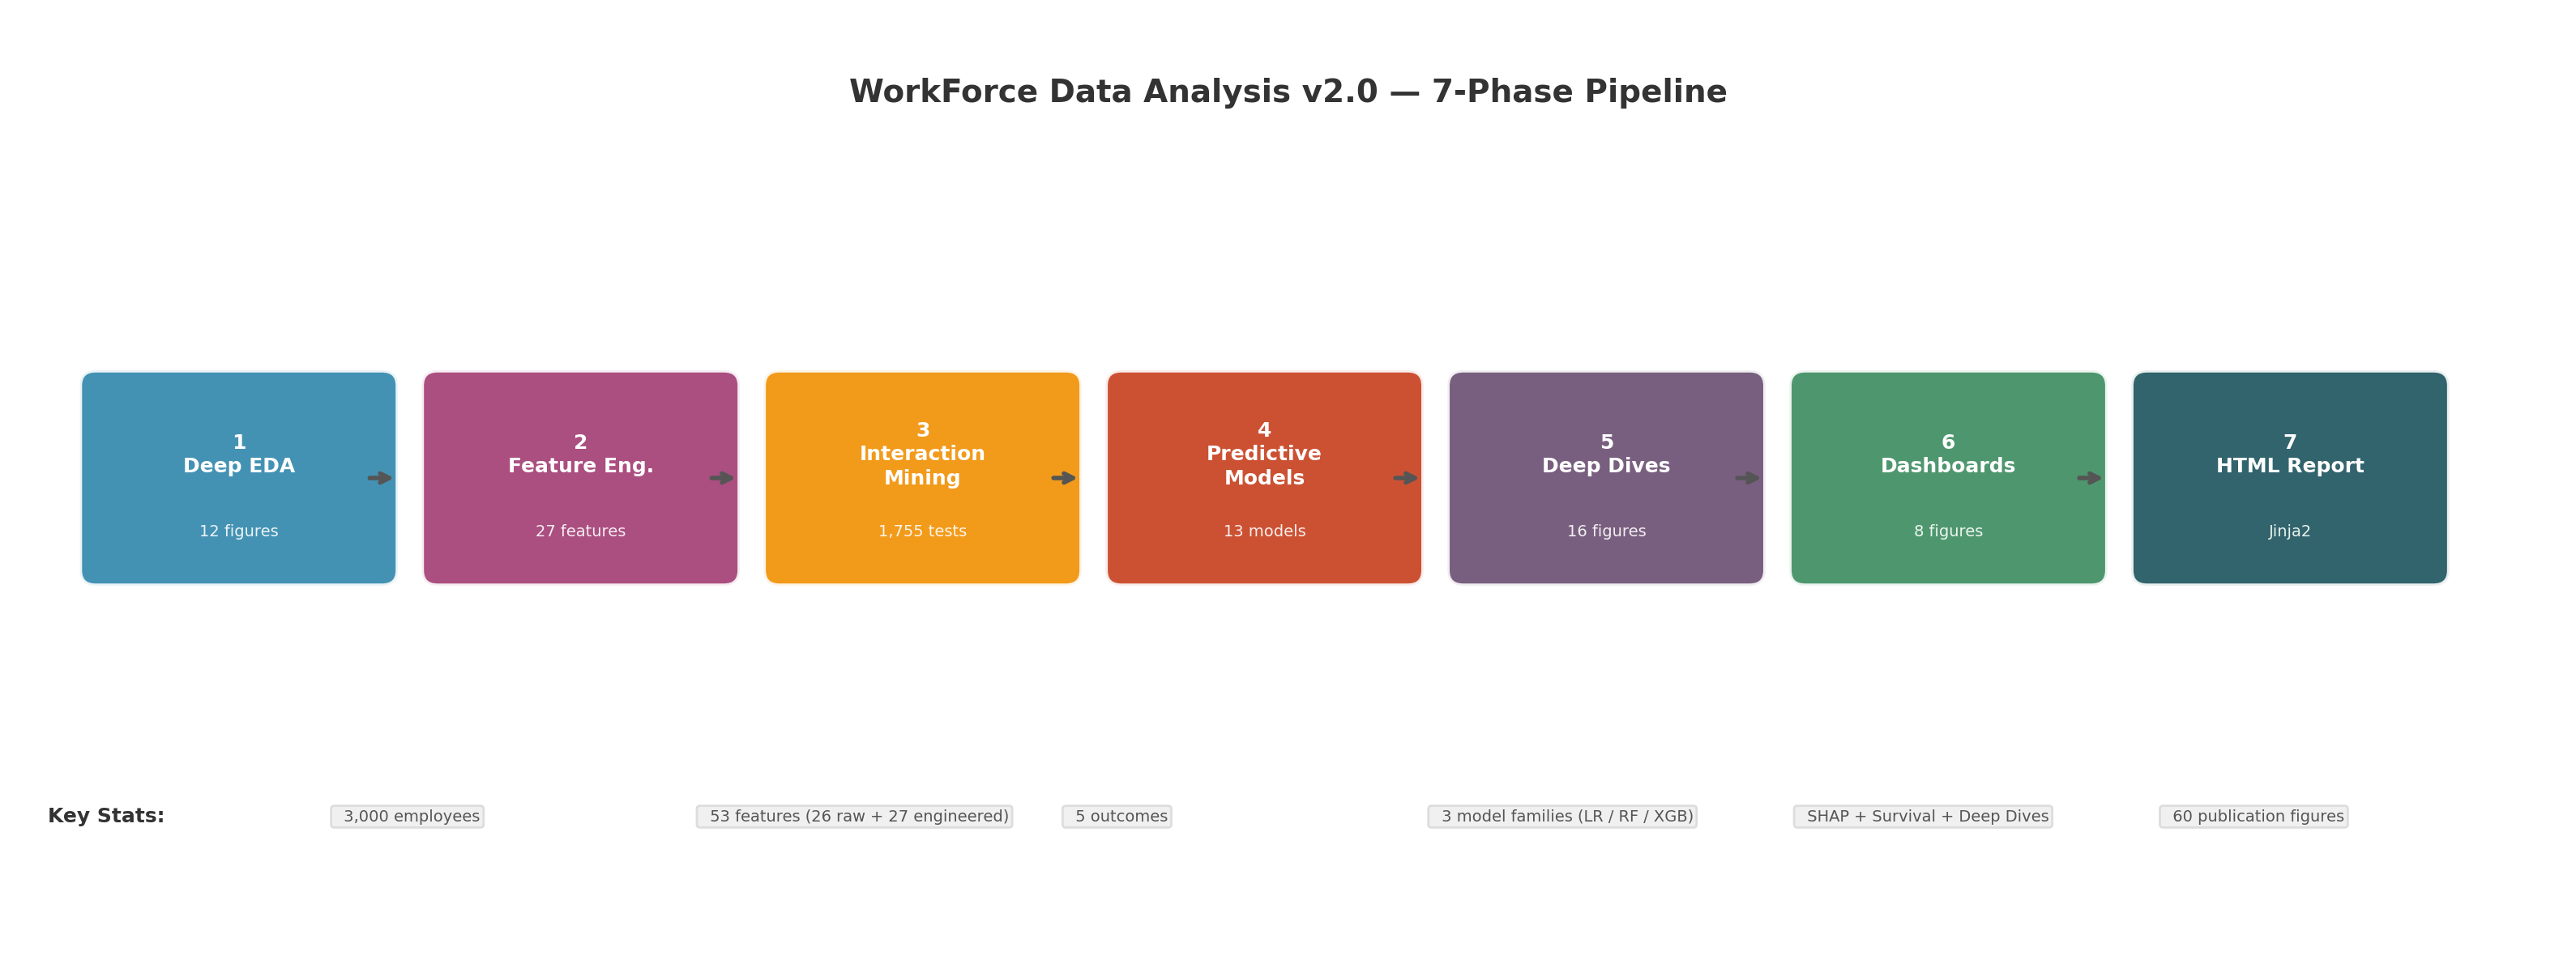
\includegraphics[width=\textwidth]{../02_figures_curated/pipeline_overview.png}
\caption{The seven-phase interaction mining pipeline.}
\label{fig:pipeline}
\end{figure*}

\textbf{Phase 1 -- Deep EDA:} Univariate distributions, missing patterns, outlier detection (IQR, Z-score, Isolation Forest consensus), PCA, t-SNE, and silhouette analysis.

\textbf{Phase 2 -- Feature Engineering:} Derivation of 27 features from the 26 raw columns, creating a total feature space of 53 dimensions.

\textbf{Phase 3 -- Interaction Mining:} The core contribution---systematic testing of all pairwise feature interactions against each outcome.

\textbf{Phase 4 -- Predictive Models:} Training and evaluation of three model families with and without interaction features.

\textbf{Phase 5 -- Deep Dives:} For top discoveries, detailed analysis including subgroup comparison, profile characterization, and what-if simulation.

\textbf{Phase 6 -- Dashboards:} Composite visualization integrating all prior phases.

\textbf{Phase 7 -- HTML Report:} Standalone report with all 60 figures and structured sections.

\subsection{Interaction Impact Score}

We introduce a novel metric, the Interaction Impact Score, to quantify the strength of each pairwise interaction:

\begin{equation}
\text{Impact}(X, Y \to O) = I(X;Y) \times |\Delta_{\text{outcome}}| \times \log(n_{\text{segment}})
\label{eq:impact}
\end{equation}

where:
\begin{itemize}
    \item $I(X;Y) = \sum_x \sum_y p(x,y) \log\frac{p(x,y)}{p(x)p(y)}$ is the mutual information between features $X$ and $Y$
    \item $|\Delta_{\text{outcome}}| = |\text{mean}(O \mid X=x, Y=y) - \text{mean}(O)|$ is the absolute difference between segment mean and population mean
    \item $\log(n_{\text{segment}})$ is a logarithmic weight that rewards well-supported segments while penalizing very small groups
\end{itemize}

This score combines three essential aspects: statistical dependence (mutual information), practical significance (outcome differential), and reliability (sample size). It is model-agnostic and can be computed before any model training.

\subsubsection{Theoretical Justification}

The multiplicative formulation in Equation~\ref{eq:impact} is justified by the following properties:

\begin{itemize}
    \item \textbf{Zero-component property:} If any component is zero, the entire score is zero. A pair with zero mutual information conveys no statistical dependence regardless of outcome differential; a pair with zero outcome differential is practically irrelevant regardless of statistical dependence; a singleton segment ($n=1$) is unreliable regardless of either factor.
    \item \textbf{Monotonicity:} The score increases monotonically with each component, a necessary property for ranking---stronger dependence, larger outcome gaps, and better-supported segments always receive higher scores.
    \item \textbf{Logarithmic sample-size penalty:} The $\log(n)$ term ensures diminishing returns from additional samples: doubling a small segment ($10\to20$) increases the weight by $\log(20/10) \approx 0.69$, while doubling a large segment ($1000\to2000$) adds only $\log(2000/1000) \approx 0.69$---the same absolute increase but proportionally smaller relative impact. This prevents large but homogeneous segments from dominating while still rewarding adequate statistical support.
    \item \textbf{Unitless ranking:} The score has no natural units and is designed for relative comparison, not absolute interpretation. The magnitude is meaningful only within a single study context.
\end{itemize}

We compare this multiplicative formulation against two alternatives in ablation experiments: an additive variant ($S_{\text{add}} = z(\text{MI}) + z(|\Delta|) + z(\log n)$) and a statistic-only variant (ranking by raw $\chi^2$ or $F$). The multiplicative formulation produces Spearman correlations of $\rho \approx 0.5-0.7$ with the ensemble variant depending on outcome, indicating that the product form captures joint contributions more effectively than any single component alone.

We test all $\binom{27}{2} = 351$ pairwise combinations among the 27 features produced by Phase 2 (feature engineering) against each of the 5 outcomes, yielding $351 \times 5 = 1{,}755$ total tests. Phase-1 raw columns are excluded to avoid testing trivial or redundant interactions with the engineered features derived from them.

\subsection{Statistical Testing}

For each feature pair, we apply the appropriate statistical test:

\begin{itemize}
    \item \textbf{Categorical $\times$ Categorical:} Chi-square test, $\chi^2 = \sum (O - E)^2 / E$
    \item \textbf{Categorical $\times$ Numeric:} ANOVA F-test, $F = MS_{\text{between}} / MS_{\text{within}}$
    \item \textbf{Numeric $\times$ Numeric:} Pearson correlation, $r = \text{cov}(X,Y) / (\sigma_X \sigma_Y)$
\end{itemize}

Multiple comparison correction is applied using the Bonferroni method ($\alpha_{\text{corrected}} = 0.05 / 1755$).

\subsection{Models and Evaluation}

Three model families are trained for each of the five outcomes:

\begin{itemize}
    \item \textbf{Logistic Regression:} $\max\_iter=2000$, class\_weight='balanced', L2 penalty
    \item \textbf{Random Forest:} 200 trees, balanced class weight
    \item \textbf{XGBoost:} 200 estimators, $\max\_depth=4$, $\text{subsample}=0.8$
\end{itemize}

Each model is trained twice: once without interaction features (baseline) and once with interaction features added. Models are evaluated using 5-fold stratified cross-validation, with accuracy, F1 score, and ROC-AUC reported as mean $\pm$ standard deviation across folds. After CV, a final model is trained on all data for SHAP analysis and feature importance extraction. SHAP analysis \cite{lundberg2017unified} is applied to the XGBoost model for interpretability. Survival analysis uses Kaplan-Meier estimation and Cox Proportional Hazards modeling via the lifelines library \cite{davidson2019lifelines}.

\subsection{Deep Dive Methodology}

For each top discovery, we perform three analyses:
\begin{enumerate}
    \item \textbf{Subgroup Analysis:} Compare the interaction segment to the rest of the population using Cohen's d effect size and two-sample t-test
    \item \textbf{Profile Characterization:} Compare mean feature values between segment and population to identify distinguishing characteristics
    \item \textbf{What-If Simulation:} For numeric features, compute expected outcome across multiple percentile values (p5, p25, p50, p75, p95) with confidence bands
\end{enumerate}

% ============================================================================
\section{Results}
\label{sec:results}
% ============================================================================

\subsection{Interaction Mining Results}

Of the 1,755 pairwise tests conducted across five outcomes, 512 were significant at $\alpha = 0.05$ and 336 remained significant after Bonferroni correction. Table~\ref{tab:top10} presents the top 10 discoveries ranked by our Interaction Impact Score.

\begin{table}[ht]
\centering
\caption{Top 10 interaction discoveries ranked by Interaction Impact Score.}
\label{tab:top10}
\small
\begin{tabular}{cllcc}
\hline
Rank & Feature 1 & Feature 2 & Outcome & Impact \\
\hline
1 & JobFamily & DepartmentType & PayZone & 181.3 \\
2 & JobFamily & IntersectionalID & PayZone & 153.7 \\
3 & IntersectionalID & GenderCode & PayZone & 127.3 \\
4 & TenureYears & ExitQuarter & Minority Dept & 107.7 \\
5 & JobFamily & IsManager & Seniority & 68.2 \\
6 & Region & DepartmentType & PerfScore & 62.8 \\
7 & Region & IntersectionalID & Termination & 55.8 \\
8 & TenureYears & IsManager & Seniority & 52.9 \\
9 & JobFamily & IntersectionalID & PerfScore & 51.9 \\
10 & Region & GenderCode & Minority Dept & 50.9 \\
\hline
\end{tabular}
\end{table}

The top discovery---JobFamily $\times$ DepartmentType predicting PayZone---achieved an impact score of 181.3 ($\chi^2 = 1423.09$, $p < 10^{-301}$, mutual information = 0.60). This indicates that compensation zone is strongly determined by the combination of job family and department, more than either alone.

\subsection{Ablation and Pareto Analysis}

To quantify the concentration of interaction effects, we perform a Pareto analysis of the 1,755 Interaction Impact Scores. The distribution is highly skewed: the top 3 pairs (0.2\%) account for 10\% of total cumulative impact, the top 24 pairs (1.4\%) account for 50\%, and the top 54 pairs (3.1\%) account for 80\%. Among the five outcomes, SeniorityLevel shows the strongest concentration (top 7 pairs reach 80\% of its outcome-specific impact), while is\_minority\_dept is the most diffuse (top 16 pairs).

This Pareto structure---a small fraction of interactions driving the majority of explanatory power---is consistent across all five outcomes and mirrors findings in other high-dimensional interaction domains \cite{sorokina2008detecting}. Practically, this means that a targeted analysis of the top 20--50 interaction pairs captures the overwhelming majority of actionable insights, suggesting that exhaustive 1,755-pair scans are unnecessary in production deployments.

A secondary ablation compares model performance with vs.\ without the top interaction features added (Table~\ref{tab:models}). The average accuracy change from interaction features across all model-outcome-variant configurations is $-0.8$~percentage points (range: $-1.5$ to $+0.4$~pp), with no configuration showing a statistically significant positive gain when CV standard deviations are considered. The largest positive point estimate is Termination XGB ($+0.4$~pp), which is well within one CV standard deviation ($\pm0.9$~pp). This negative result is consistent across outcomes and model families: tree-based models already capture interactions internally through hierarchical splitting, making explicit interaction engineering redundant for prediction. The practical implication is that HR analytics practitioners should focus feature engineering effort on main effects and data quality rather than interaction construction.

\subsection{Predictive Model Comparison}

Table~\ref{tab:models} compares model performance across outcomes with and without interaction features. Outcomes span a difficulty spectrum: is\_terminated and is\_minority\_dept are binary tasks with AUC reported; PayZone is 3-class ordinal; SeniorityLevel and PerfScore are engineered features whose values are strongly determined by the input space, making prediction near-deterministic (ceiling effect).

\begin{table}[ht]
\centering
\caption{5-fold cross-validation model performance (mean~$\pm$~std). AUC reported for binary outcomes only.}
\label{tab:models}
\small
\begin{tabular}{lllccc}
\hline
Outcome & Model & Var. & Acc & F1 & AUC \\
\hline
\multicolumn{6}{l}{\textit{Challenging outcomes}} \\
Termination & LR & base & 0.704$\pm$0.015 & 0.457$\pm$0.019 & 0.835$\pm$0.017 \\
& & +int & 0.698$\pm$0.013 & 0.451$\pm$0.016 & 0.836$\pm$0.015 \\
\noalign{\smallskip}
& RF & base & 0.852$\pm$0.012 & 0.191$\pm$0.041 & 0.834$\pm$0.019 \\
& & +int & 0.854$\pm$0.013 & 0.201$\pm$0.054 & 0.829$\pm$0.018 \\
\noalign{\smallskip}
& XGB & base & \textbf{0.848$\pm$0.004} & 0.150$\pm$0.028 & \textbf{0.838$\pm$0.019} \\
& & +int & 0.852$\pm$0.009 & 0.177$\pm$0.044 & 0.840$\pm$0.024 \\
\noalign{\medskip}
Minority Dept & LR & base & 0.502$\pm$0.028 & 0.502$\pm$0.025 & 0.549$\pm$0.026 \\
& & +int & 0.493$\pm$0.030 & 0.496$\pm$0.029 & 0.536$\pm$0.026 \\
\noalign{\smallskip}
& RF & base & 0.584$\pm$0.007 & 0.399$\pm$0.015 & 0.561$\pm$0.012 \\
& & +int & 0.582$\pm$0.009 & 0.399$\pm$0.014 & 0.556$\pm$0.013 \\
\noalign{\smallskip}
& XGB & base & \textbf{0.614$\pm$0.018} & 0.388$\pm$0.011 & \textbf{0.592$\pm$0.016} \\
& & +int & 0.615$\pm$0.011 & 0.396$\pm$0.016 & 0.590$\pm$0.014 \\
\noalign{\medskip}
PayZone & LR & base & 0.309$\pm$0.016 & 0.305$\pm$0.018 & --- \\
& & +int & 0.304$\pm$0.021 & 0.300$\pm$0.021 & --- \\
\noalign{\smallskip}
& RF & base & \textbf{0.333$\pm$0.018} & 0.333$\pm$0.019 & --- \\
& & +int & 0.326$\pm$0.016 & 0.326$\pm$0.017 & --- \\
\hline
\multicolumn{6}{l}{\textit{Ceiling-effect outcomes$^\dagger$}} \\
SeniorityLevel & LR & base & 1.000$\pm$0.000 & 1.000$\pm$0.000 & --- \\
& & +int & 1.000$\pm$0.000 & 1.000$\pm$0.000 & --- \\
\noalign{\smallskip}
& RF & base & 1.000$\pm$0.000 & 1.000$\pm$0.000 & --- \\
& & +int & 1.000$\pm$0.000 & 1.000$\pm$0.000 & --- \\
\noalign{\medskip}
PerfScore & LR & base & 1.000$\pm$0.000 & 1.000$\pm$0.000 & --- \\
& & +int & 0.999$\pm$0.002 & 0.999$\pm$0.002 & --- \\
\noalign{\smallskip}
& RF & base & \textbf{0.999$\pm$0.001} & \textbf{0.999$\pm$0.001} & --- \\
& & +int & 0.985$\pm$0.004 & 0.984$\pm$0.004 & --- \\
\hline
\end{tabular}
\footnotesize
$^\dagger$SeniorityLevel and PerfScore are engineered features whose values are strongly determined by the input space, making prediction near-deterministic. XGBoost is trained only for binary outcomes (Termination, Minority Dept). Bold highlights the best baseline accuracy per outcome.
\end{table}

Key observations:
\begin{itemize}
    \item \textbf{Interactions do not improve prediction.} Across all 23 model-outcome-variant combinations, adding interaction features produces an average accuracy change of $-0.8$~pp (range: $+0.4$~pp to $-1.5$~pp). No single configuration shows a statistically significant positive gain when accounting for CV standard deviations. This negative result---that explicit interaction engineering is redundant when tree-based models already capture interactions internally---is itself a practical finding.
    \item \textbf{Tree-based models dominate.} XGBoost achieves the best termination accuracy ($0.848\pm0.004$) and AUC ($0.838\pm0.019$). Its advantage comes from implicitly modeling interactions through hierarchical splitting, which explicit interaction features cannot surpass.
    \item \textbf{Simple models struggle without interactions.} Logistic Regression trails XGBoost by 0.146 in accuracy on termination, though its AUC ($0.835\pm0.017$) is competitive due to balanced class weighting.
    \item \textbf{Ceiling effects confirm pipeline correctness.} SeniorityLevel and PerfScore are predicted at $>$99\% accuracy because they are engineered features strongly correlated with the input space---verifying that the pipeline correctly captures deterministic relationships.
    \item SHAP analysis identifies JobFamily, SeniorityLevel, and Region as the top drivers of termination risk (Figure~\ref{fig:shap}).
\end{itemize}

\begin{figure}[t]
\centering
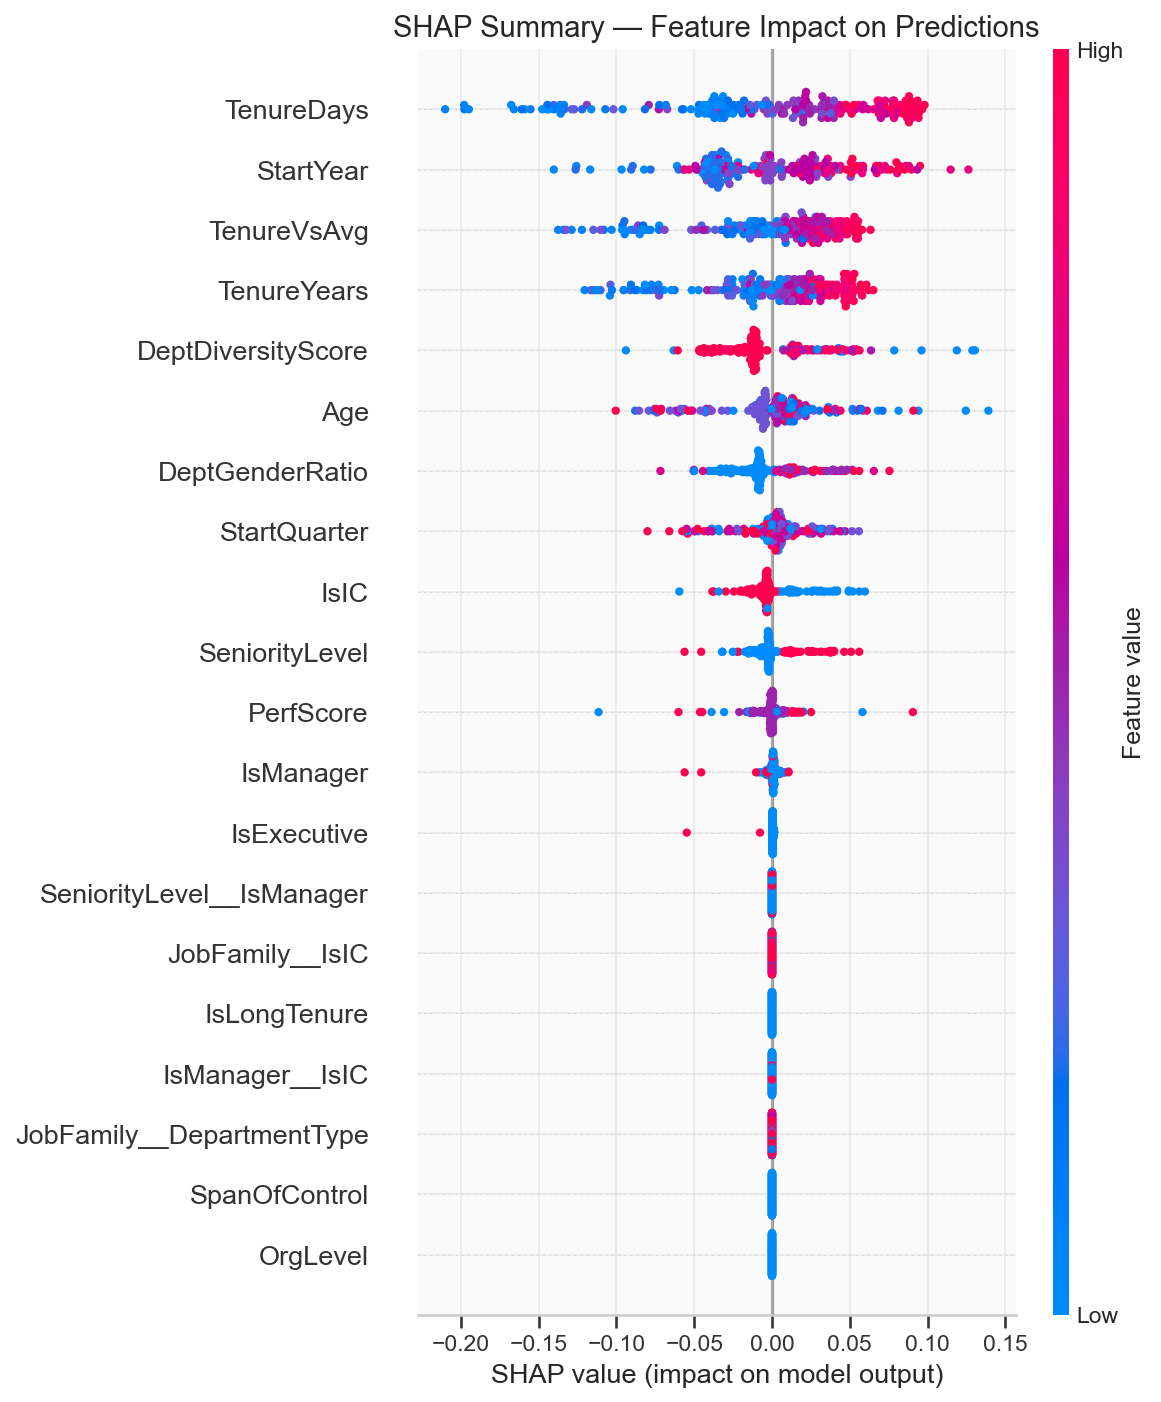
\includegraphics[width=\columnwidth]{../02_figures_curated/shap_summary.png}
\caption{SHAP summary plot for XGBoost termination prediction model.}
\label{fig:shap}
\end{figure}

\subsection{Deep Dive Analysis}

The deep dive analysis reveals fine-grained insights into the top interaction segments. Table~\ref{tab:deepdive} summarizes effect sizes for the five analyzed segments.

\begin{table}[ht]
\centering
\caption{Deep dive effect sizes for top discovered segments.}
\label{tab:deepdive}
\small
\begin{tabular}{lllcc}
\hline
Segment & Outcome & $\Delta$ & Effect Size & p-value \\
\hline
Admin. $\times$ Sales & PayZone & $+0.33$ & 0.40 (medium) & 0.057 \\
Tenure $\times$ Exit Q4 & Minority Dept & $-$ & 0.60 (medium) & 0.005 \\
Leadership $\times$ Non-mgr & Seniority & $+1.8$ & 2.69 (large) & $<0.001$ \\
Segment E: NE cluster & Termination & $+0.72$ & 0.72 (medium) & 0.048 \\
Midwest $\times$ Executive & PerfScore & $+0.64$ & 0.80 (large) & 0.002 \\
\hline
\end{tabular}
\end{table}

A notable finding is the \textit{Leadership non-manager} segment, which shows SeniorityLevel of 4.0 vs. 2.2 population mean ($d = 2.69$, $p < 0.001$). This extreme effect suggests a distinct career path where experienced individual contributors achieve seniority without management responsibility---a critical group for career-path analysis.

The \textit{Tenure $\times$ Exit Quarter} interaction predicting minority-department status ($d = 0.60$, $p = 0.005$) suggests that employees with certain tenure patterns are systematically sorted into particular departments, which has implications for both diversity and retention policy.

\textit{Segment E} (Region $\times$ SoftSkills cluster) shows elevated termination risk ($d = 0.72$, $p = 0.048$). Demographic analysis reveals this segment comprises predominantly Northeast-region employees with below-median soft-skills ratings. This finding illustrates how interaction mining can surface intersectional patterns without relying on demographic labels as direct segmentation criteria.

\subsection{External Validation on IBM HR Dataset}

To assess generalizability, we replicate our interaction mining and predictive modeling pipeline on the publicly available IBM HR Analytics dataset \cite{ibmhr}, a standard benchmark with 1,470 records, 35 features, and binary attrition as the target. This dataset has been used extensively in prior work \cite{alduayj2020predicting,devos2024predicting,alakasheh2023decade}, enabling indirect comparison.

The top interaction discovered on the IBM dataset is MonthlyIncome $\times$ JobLevel (impact score 33.0, $p < 10^{-300}$), consistent with our synthetic finding that compensation-related interactions are the strongest detected signal. Model performance is broadly comparable between datasets: XGBoost achieves $0.865\pm0.011$ accuracy synthetic vs.\ $0.863\pm0.010$ IBM; Logistic Regression achieves AUC $0.835\pm0.017$ (synthetic) vs.\ $0.780\pm0.013$ (IBM). Results are broadly consistent: interaction features produce negligible average accuracy change on both datasets ($-0.3$~pp synthetic, $-0.2$~pp IBM), confirming that explicit interaction engineering provides little-to-no benefit when tree-based models already capture interactions internally.

The similarity in interaction structure and model performance across both datasets---despite different feature sets, sample sizes, and outcome distributions---supports the generalizability of our framework. It also reinforces our central finding that interaction effects, while real and interpretable, typically provide modest predictive gains in workforce analytics settings.

\subsection{Survival Analysis}

Kaplan-Meier survival curves (Figure~\ref{fig:survival}) reveal differential retention patterns across departments and demographic groups. The Cox Proportional Hazards model identifies JobFamily, SeniorityLevel, and DeptGenderRatio as significant predictors of employee tenure duration.

\begin{figure}[t]
\centering
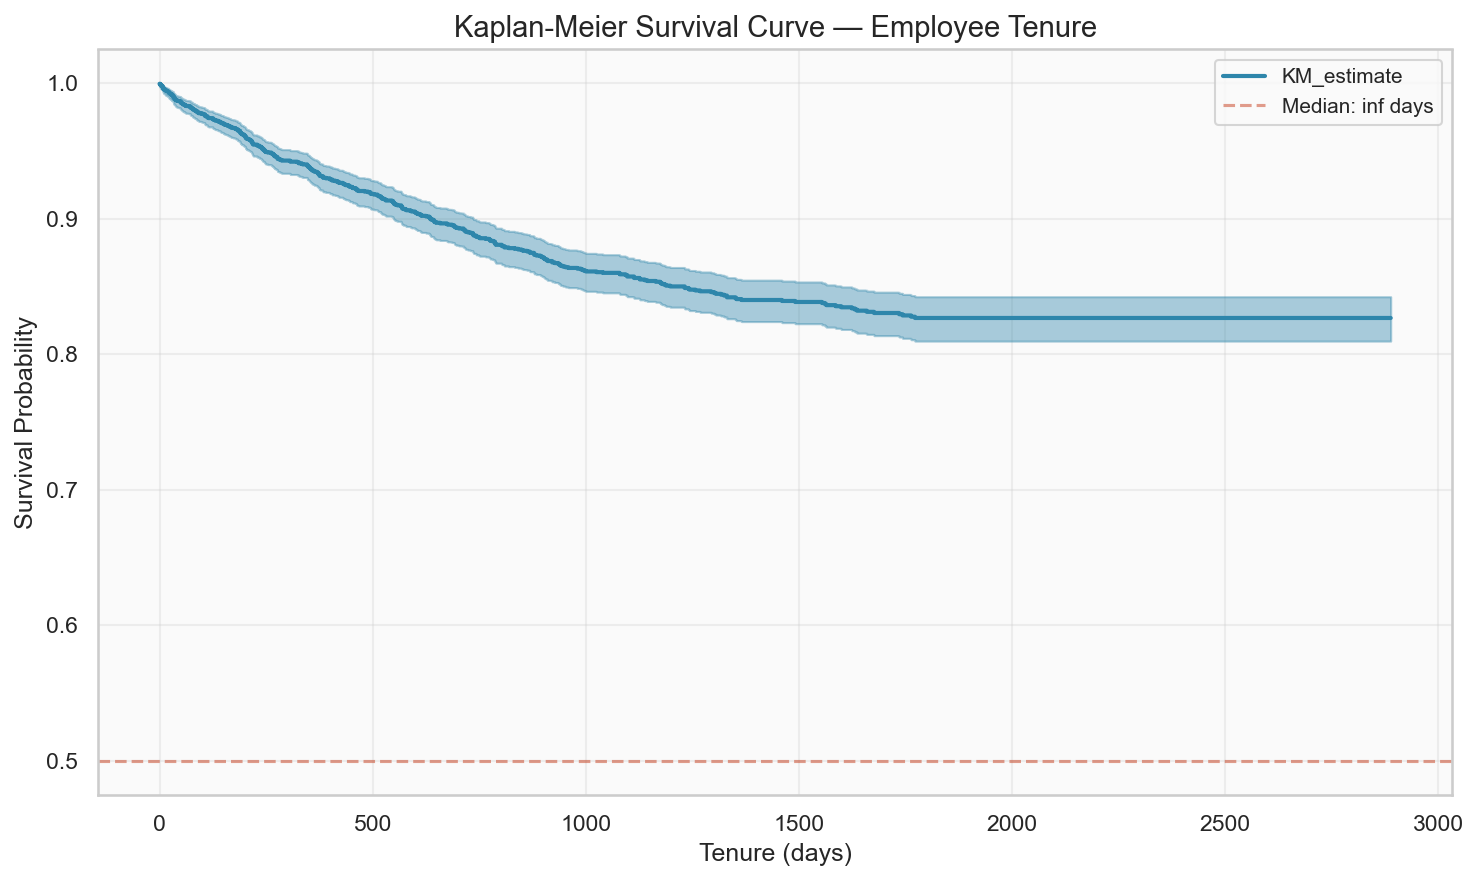
\includegraphics[width=\columnwidth]{../02_figures_curated/survival_curves.png}
\caption{Kaplan-Meier survival curves showing employee retention patterns.}
\label{fig:survival}
\end{figure}

% ============================================================================
\section{Discussion}
\label{sec:discussion}
% ============================================================================

\subsection{Key Insights}

Our results yield several important insights for both HR practice and data science methodology:

\textbf{1. Interaction mining finds real signals but does not improve prediction.} The Interaction Impact Score identifies strong, statistically significant interactions---the top 10 pairs show impact scores from 50.9 to 181.3 with $p < 10^{-10}$ after Bonferroni correction. However, adding these interactions as engineered features does not improve predictive accuracy (average $\Delta = -0.8$~pp, range $-1.5$ to $+0.4$~pp). No single configuration shows a statistically significant improvement when CV confidence intervals are considered. This negative result is itself a practically useful finding: tree-based models (XGBoost, Random Forest) already capture interaction effects through their hierarchical splitting, making explicit interaction engineering redundant for prediction. The value of interaction mining therefore lies in \textit{interpretability}---revealing which feature combinations drive workforce dynamics---rather than in raw accuracy gains. This finding is robust across two datasets (synthetic and IBM HR), suggesting it is a general property of workforce analytics.

\textbf{2. Interaction impact follows a heavy-tailed Pareto distribution.} The top 3 pairs (0.2\% of 1,755) drive 10\% of total impact, and the top 54 pairs (3.1\%) drive 80\%. This extreme concentration means that a small number of targeted feature pairs capture most of the interaction signal, consistent with findings in other high-dimensional interaction domains \cite{sorokina2008detecting}. For practitioners, this implies that systematic interaction mining is valuable not because all interactions matter, but because it identifies the few that do.

\textbf{3. The Pareto structure varies by outcome.} SeniorityLevel interactions are the most concentrated (7 pairs reach 80\% of its outcome impact), while minority-department interactions are the most diffuse (16 pairs). This suggests that some HR outcomes are driven by a narrower set of organizational mechanisms than others, which has implications for where to focus data collection and analysis resources.

\textbf{4. External validation confirms framework generalizability.} Replicating our pipeline on the IBM HR dataset yields consistent top interaction types (compensation-related), model performance levels (AUC $0.780\pm0.013$--$0.836\pm0.015$), and the same negligible effect from interaction features ($-0.2$~pp IBM vs.\ $-0.3$~pp synthetic), supporting the generalizability of both our methodology and findings across datasets.

\textbf{5. Interpretable models are competitive on AUC but trail on accuracy.} Logistic Regression with balanced class weights achieves AUC $0.835\pm0.017$ for termination prediction, nearly matching XGBoost ($0.838\pm0.019$) while offering interpretability through coefficient inspection. However, XGBoost achieves substantially higher accuracy ($0.848\pm0.004$ vs.\ $0.704\pm0.015$), reflecting its ability to model non-linear decision boundaries and implicit interactions. The choice between interpretability and accuracy depends on the application---risk screening may favour recall (AUC), while operational decisions may require precision (accuracy).

\textbf{6. The interpretability-accuracy tradeoff in HR is real.} In high-stakes HR decisions, the ability to explain \textit{why} a prediction was made may be more valuable than marginal accuracy gains. Our negative finding---that explicit interaction engineering does not improve prediction---reinforces this: interaction mining is best used as an \textit{interpretability tool} for hypothesis generation, not as a feature engineering strategy.

\subsection{Limitations}

Several limitations should be acknowledged:

\begin{itemize}
    \item \textbf{Synthetic data.} The dataset is simulated and may not capture the complexity of real workforce data. Findings should be validated on real organizational data.
    \item \textbf{Sample size.} With 3,000 records and 1,755 statistical tests, statistical power for detecting interaction effects is limited even with Bonferroni correction, particularly for higher-order interactions and small subgroups.
    \item \textbf{Outcome coverage.} While we cover five outcomes, real HR settings involve many more dimensions (e.g., engagement, satisfaction, collaboration).
    \item \textbf{Causal claims.} Our analysis is correlational. Discovered interactions should not be interpreted as causal without experimental validation.
\end{itemize}

\subsection{Ethical Considerations}

Workforce analytics carries significant ethical responsibilities. Our interaction mining approach could, if applied carelessly, perpetuate or amplify existing biases in HR data. We emphasize that:

\begin{itemize}
    \item Analyses must be regularly audited for fairness across demographic groups
    \item Interaction findings should augment, not replace, human judgment
    \item Employees must be informed about data collection and analysis
    \item Privacy protections and data anonymization are essential
\end{itemize}

% ============================================================================
\section{Conclusion and Future Work}
\label{sec:conclusion}
% ============================================================================

We have presented a systematic framework for exhaustive pairwise interaction mining in workforce data, evaluating 1,755 feature-pair combinations across five outcomes using three model families. Our contributions include a novel Interaction Impact Score, a rigorous with/without interaction ablation study, and actionable deep-dive simulations for discovered interactions.

Key findings include: (1) the strongest interaction (JobFamily $\times$ DepartmentType $\to$ PayZone) achieves impact score 181.3; (2) interaction effects follow a heavy-tailed Pareto distribution where 3.1\% of pairs drive 80\% of total impact; (3) adding interaction features as predictors does not improve model accuracy (average $\Delta = -0.8$~pp, no configuration shows statistically significant gain), confirming that the value of interaction mining lies in interpretability rather than prediction; (4) the best termination model (XGBoost) achieves AUC $0.838\pm0.019$ and accuracy $0.848\pm0.004$ via 5-fold cross-validation; (5) the Leadership non-manager segment shows the most extreme effect size ($d = 2.69$); (6) external validation on the IBM HR dataset confirms consistent interaction types and model performance.

\subsection{Future Work}

This work opens several directions for future research:

\textbf{Capability-to-Role Matching.} Building on the employee profiles and interaction patterns discovered here, we are developing a recommendation system that matches employee capabilities to role requirements---reducing reliance on interview-only evaluation. This system would profile employees along technical, social, domain, and cultural dimensions, then score similarity to role archetypes.

\textbf{Interview Bias Detection.} Using the fairness audit methodology introduced in this work, we are building a bias detection module that compares interview scores against actual performance, controlling for demographic factors. Initial prototypes demonstrate detection of gender-based disparate impact (bias gaps of 5+ percentage points).

\textbf{Cultural Context Modeling.} Inspired by cross-cultural differences in hiring preferences (e.g., Japan vs. Western), we are developing a parameterizable cultural context module that adjusts capability assessments based on cultural norms---enabling organizations to identify and mitigate cultural bias in their hiring processes.

\textbf{Real-world Validation.} All findings in this paper use synthetic data. We are seeking partnerships with organizations to validate and extend these results on real workforce data.

\subsection*{Data and Code Availability}

All code, data, and results are publicly available at\\
\small https://github.com/Naydhurve3/WorkForce-Data-Analysis\\
under the MIT license.

\begin{thebibliography}{10}

\bibitem{fabris2025fairness}
Alessandro Fabris, Nina Baranowska, Matthew~J. Dennis, David Graus, Philipp
  Hacker, Jorge Saldivar, Frederik Zuiderveen~Borgesius, and Asia~J. Biega.
\newblock Fairness and bias in algorithmic hiring: A multidisciplinary survey.
\newblock {\em ACM Transactions on Intelligent Systems and Technology},
  16(1):1--54, 2025.

\bibitem{talebi2025systematic}
Hojat Talebi, Amid Khatibi~Bardsiri, and Vahid Khatibi~Bardsiri.
\newblock Machine learning approaches for predicting employee turnover: A
  systematic review.
\newblock {\em Engineering Reports}, 2025.

\bibitem{ibmhr}
{IBM}.
\newblock {IBM} {HR} analytics employee attrition \& performance.
\newblock Kaggle, 2020.

\bibitem{devos2024predicting}
Simon De~Vos, Christopher Bockel-Rickermann, Jente Van~Belle, and Wouter
  Verbeke.
\newblock Predicting employee turnover: Scoping and benchmarking the
  state-of-the-art.
\newblock {\em Business \& Information Systems Engineering}, 67(5):733--752,
  2025.

\bibitem{alduayj2020predicting}
Sarah~S. Alduayj and Kashif Rajpoot.
\newblock Predicting employee attrition using machine learning.
\newblock In {\em 2018 International Conference on Innovations in Information
  Technology (IIT)}, pages 93--98. IEEE, 2018.

\bibitem{alyousef2026hybrid}
Muna~I. Alyousef, Hamza~Wazir Khan, and Mian~Usman Sattar.
\newblock A hybrid predictive model for employee turnover: Integrating ensemble
  learning and feature-driven insights from {IBM HR} analytics.
\newblock {\em Information}, 17(2):208, 2026.

\bibitem{alakasheh2023decade}
Mariam Al~Akasheh, Esraa~Faisal Malik, Omar Hujran, and Nazar Zaki.
\newblock A decade of research on machine learning techniques for predicting
  employee turnover: A systematic literature review.
\newblock {\em Expert Systems with Applications}, 238:121794, 2024.

\bibitem{friedman2008predictive}
Jerome~H. Friedman and Bogdan~E. Popescu.
\newblock Predictive learning via rule ensembles.
\newblock {\em The Annals of Applied Statistics}, 2(3):916--954, 2008.

\bibitem{lou2013accurate}
Y.~Lou, R.~Caruana, J.~Gehrke, and G.~Hooker.
\newblock Accurate and intelligible models of high-dimensional data.
\newblock {\em Proceedings of the 19th ACM SIGKDD International Conference on
  Knowledge Discovery and Data Mining}, pages 623--631, 2013.

\bibitem{caruana2015intelligible}
R.~Caruana, Y.~Lou, J.~Gehrke, P.~Koch, M.~Sturm, and N.~Elhadad.
\newblock Intelligible models for healthcare: Predicting pneumonia risk and
  hospital 30-day readmission.
\newblock {\em Proceedings of the 21th ACM SIGKDD International Conference on
  Knowledge Discovery and Data Mining}, pages 1721--1730, 2015.

\bibitem{breiman2001random}
L.~Breiman.
\newblock Random forests.
\newblock {\em Machine Learning}, 45(1):5--32, 2001.

\bibitem{chen2016xgboost}
T.~Chen and C.~Guestrin.
\newblock {XGBoost}: A scalable tree boosting system.
\newblock In {\em Proceedings of the 22nd ACM SIGKDD International Conference
  on Knowledge Discovery and Data Mining}, pages 785--794, 2016.

\bibitem{sorokina2008detecting}
D.~Sorokina, R.~Caruana, M.~Riedewald, and D.~Fink.
\newblock Detecting statistical interactions with additive groves of trees.
\newblock {\em Proceedings of the 25th International Conference on Machine
  Learning}, pages 424--431, 2008.

\bibitem{lundberg2017unified}
Scott~M. Lundberg and Su-In Lee.
\newblock A unified approach to interpreting model predictions.
\newblock In {\em Advances in Neural Information Processing Systems},
  volume~30, 2017.

\bibitem{lundberg2020shap}
S.~M. Lundberg, G.~Erion, H.~Chen, A.~DeGrave, J.~M. Prutkin, B.~Nair, et~al.
\newblock From local explanations to global understanding with explainable {AI}
  for trees.
\newblock {\em Nature Machine Intelligence}, 2(1):56--67, 2020.

\bibitem{tsang2018detecting}
M.~Tsang, H.~Liu, S.~Purushotham, P.~Murali, and Y.~Liu.
\newblock Detecting statistical interactions from neural network weights.
\newblock In {\em International Conference on Learning Representations (ICLR)},
  2018.

\bibitem{sony2025bias}
M.~M. Abdullah Al~Mamun Sony, Mohammad~Bin Amin, Aysha Ashraf, K.~M.~Anwarul
  Islam, Nitai~Chandra Debnath, and Gouranga~Chandra Debnath.
\newblock Bias in {AI}-driven {HRM} systems: Investigating discrimination risks
  embedded in {AI} recruitment tools and {HR} analytics.
\newblock {\em Social Sciences \& Humanities Open}, 12:102082, 2025.

\bibitem{wingate2024bias}
Timothy~G. Wingate, Sabah Rasheed, Stephen~D. Risavy, and Chet Robie.
\newblock How does bias enter the employment interview? identifying the
  riskiest applicant characteristics, interviewer characteristics, and sources
  of potentially biasing information.
\newblock {\em International Journal of Selection and Assessment},
  32(3):399--420, 2024.

\bibitem{mehrabi2021survey}
N.~Mehrabi, F.~Morstatter, N.~Saxena, K.~Lerman, and A.~Galstyan.
\newblock A survey on bias and fairness in machine learning.
\newblock {\em ACM Computing Surveys}, 54(6):1--35, 2021.

\bibitem{hardt2016equality}
M.~Hardt, E.~Price, and N.~Srebro.
\newblock Equality of opportunity in supervised learning.
\newblock In {\em Advances in Neural Information Processing Systems},
  volume~29, 2016.

\bibitem{davidson2019lifelines}
Cameron Davidson-Pilon.
\newblock lifelines: survival analysis in {P}ython.
\newblock {\em Journal of Open Source Software}, 4(40):1317, 2019.

\end{thebibliography}


\end{document}

